%\section{Description of the hardware structure and functionality}
In the following section, the hardware parts and functions will be introduced and described. The following part consists of sensor selection, ADC, chipKIT Uno32 board, motor-shield including the H bridge, and the bluetooth transmitter.

\section{Hardware diagram}
The micro-controller is connected to the motor-shield and the motor-shield is then powering both motor 1 and motor 2. The micro-controller reads data from the sensor array every 25 microsecond by utilizing the ADC, the micro-controller then sends it further to the bluetooth unit. The bluetooth unit then sends its data to the terminal. 
\begin{figure}[!ht]
	\centering
	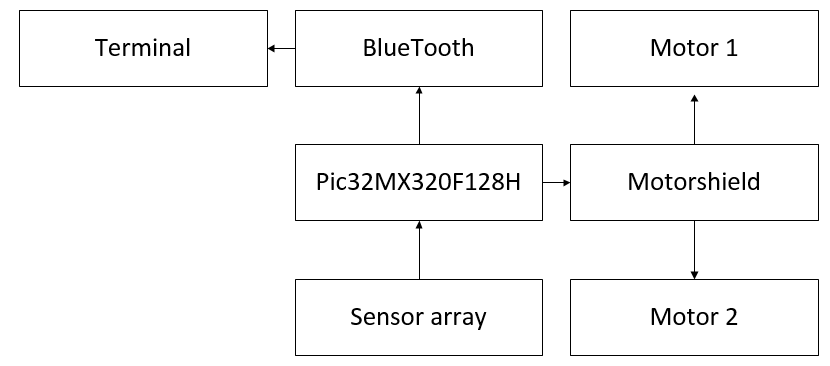
\includegraphics[width=.6\textwidth]{figures/hardwaredia.png}
	\caption{\text{Block diagram showing the hardware.}}
	\label{Hardware diagram}
\end{figure}
    
\section{Selection of sensor}
\begin{table}[]
	\centering
	\label{Sensor table}
	\begin{tabular}{|l|l|l|}
		\hline
		Name                & QRE1113 Board & OPB704    \\ \hline
		Max sensor distance & 3mm           & 3.8mm     \\ \hline
		Forward current     & 50mA          & 40mA      \\ \hline
		Mounting            & On a PCB      & In casing \\ \hline
		Price               & 19.43DKK      & 42.55DKK  \\ \hline
	\end{tabular}
	\caption{Table showing the sensors in consideration}
\end{table}
The table shows a comparison of the two sensors that were taken into consideration for the project, this is to show the price difference and the specification differences from sensor to sensor. \emph{(fig 2.1)}

\subsection{The OPB704}
The OPB704 sensor ended up being selected for the robot over the popular QRE1113 sensor board. It has a higher sensor max distance (3.8mm\footnote{http://www.farnell.com/datasheets/1884910.pdf} compared to the QRE1113s 3mm) and it has the same functionality. The way the sensor works is an LED shoots It comes with a special casing, for which a special mounting unit was 3D-printed to accommodate an array of 7. This makes the mounting very solid and tightly fitted unto the robot, which ideally makes the sensor array more stable in case of an uneven test course.
\sidebyimg{figures/opb704.jpg}{The sensor OPB 704}{figures/sensorarray.jpg}{3D printed sensor array module}

\subsection{The QRE1113 board}
Another possible sensor selection would be the QRE1113\footnote{http://cdn.sparkfun.com/datasheets/Sensors/Proximity/QRE1113.pdf} board sensor. This sensor comes complete with mounting and the necessary printing and wiring. This makes working with the sensor fairly straightforward. Although this sensor is commonly used for line following robots, when it was compared to the OPB704, it quickly became apparent that the difference in max sensor distance could become a liability, and with this in mind, the OPB704 sensor was selected.

\sidebyimg{figures/QRE.jpg}{QRE1113 Sensor on a breakout board}{figures/QREmount.jpg}{3D printed sensor array module withe the QRE1113}

\section{Analog-to-digital converter (ADC)}
The purpose of the ADC is to convert the analog signal from the sensors to digital data that can be managed by a computer - the digital data is sent through the bluetooth transmitter to a computer which displays these data readings in a GUI that has been programmed for this robot. This allows the user to read and understand what the sensors are reacting to. The sensors themselves cannot discern what signals are relevant and when to send these, the sensors just read anything they can see and send that signal. Analog signals can have a significant amount of noise - since any received noise is interpreted as part of the signal, 

*a digital signal is not only more easy to work with, it will also provide more precise data. This will make for more accurate readings on the tachometer of the robot, which allows even more finely tuned monitoring of the robot and its working processes.* TBD \\

\subsubsection{ADC diagram} 
\img{figures/ADCblock.png}{PIC32 ADC fuctional block diagram}{adcblockdiagram}{1}

\subsubsection{This products usage of ADC}
The usage of the ADC in the system, is to measure the returning voltage from the OPB704 sensor. Both the OPB704 and the QRE1113 sensors are reflective phototransistors.
A reflective phototransistor consists of a infrared LED and a phototransistor.
The phototransitors output voltage is controlled by the amount of light from the LED that is being reflected off the given surface the sensor is pointed at, back to the phototransistor.
\img{figures/reflectivesensorworkings.png}{The difference in reflection on light and dark surfaces}{reflectivesensorworkings}{0.8}

\section{The chipKIT Uno32 board}
Our main computing core is at the chipKIT Uno32 board. The board was selected based on on previous experiences, and because it meets the set requirements - most importantly it has twelve analog imputs to handle our array of seven sensors. This board utilizes the PIC32MX320F128 microcontroller, which features a 32-bit processing core running at 80MHz with 128KB of flash program memory and 16KB SRAM data memory\footnote{http://www.microchip.com/wwwproducts/en/PIC32MX320F128H}. 

*This board allowed the most important aspects of the project to become reality; namely a GUI showing both the ADC readings as well as visualizing the sensor imputs* TBD

, plenty of analog inputs to allow for the sensor array, and BlueTooth transmission of data from the robot unto a computer.\newline
The board is compatible for use with MPLAB IDE and the PICKit3 debugger.

\section{The motor shield - PKA03}
The motor shield was chosen because it is compatible with the Uno32 board, and fits perfectly within the scope of the project. It controls both motors and receives power from the 6.0 V battery pack mounted on the chassis itself. The motor shield is instrumental in providing motor controls to the product. To do this, it utilizes a specific electric circuit, called an H bridge.

\subsection{The H bridge}
An H bridge is a circuit that allows a voltage to be applied across a load in either direction. The purpose of this in the case of this project is to enable controls of the two motors in a way so they can both function individually, and both drive forwards and backwards.\\

*At first, there were experiments with custom prints and a purpose-built h bridge on the first iteration of the motor shield. However after testing, it proved faulty and was changed to accommodate time constraints.* TBD

\section{The blue-tooth transmitter - BlueSMIRF Silver}
The robot utilizes the BlueSMIRF Silver blue-tooth transceiver made by Sparkfun. Its function is to send data from the MCU (see the software section) to a C\# GUI run on a computer. This way, it is possible to monitor both the inputs the robot is receiving, as well as the logic behind the steering. It allows for any stream between 2400 to 115200 BPS\footnote{https://www.sparkfun.com/products/12577}. 
